In Figs.~(\ref{fig:distNLO1}-\ref{fig:distNLO3}), several differential distributions are shown.
All these predictions are performed at NLO accuracy at the order $\mathcal{O}(\alpha_{\rm s}\alpha^6)$.
\MP{Physics and conclusion on interference/non-factorisable etc.\ effects are not addresses yet in the discussion.}

We start with Fig.~\ref{fig:distNLO1} which displays the invariant mass (top) and the rapidity separation (bottom) of the two tagging jets.
For high invariant mass, all predictions agree rather well.
On the other hand, for low invariant mass, the hierarchy present at the level of the cross section is here reproduced.
The VBS-approximated predictions ({\sc Bonsay} and the {\sc Powheg-Box}) are lower than the full calculation ({\sc MoCaNLO}+{\sc Recola}).
The full calculation is rather well approximated by the hybrid VBS approximation implemented in {\sc MadGraph5\_aMC\-@NLO}.
Finally, {\sc VBFNLO} which includes as well $s$-channel contributions provides larger predictions at low invariant mass.
For the rapidity difference between the two tagging jets, the hierarchy between the predictions is rather similar.

 \begin{figure*}[hbt!]
   \centering
   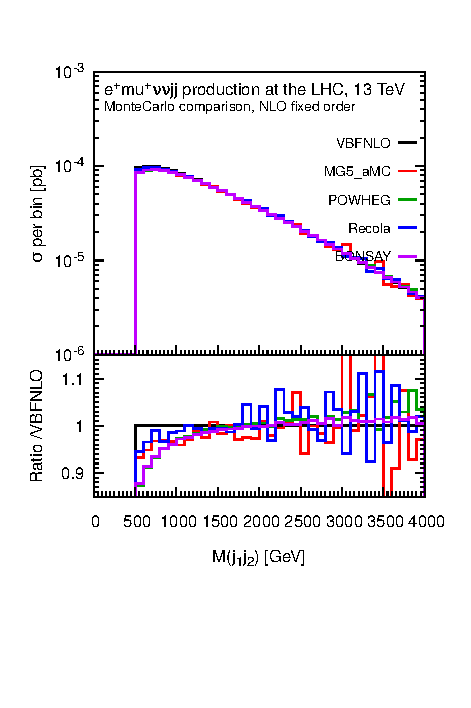
\includegraphics[width=0.4\textwidth,angle=0,clip=true,trim={0.4cm 2cm 0.cm 1.cm}]{figures/NLO/mjj_NLO.pdf}
   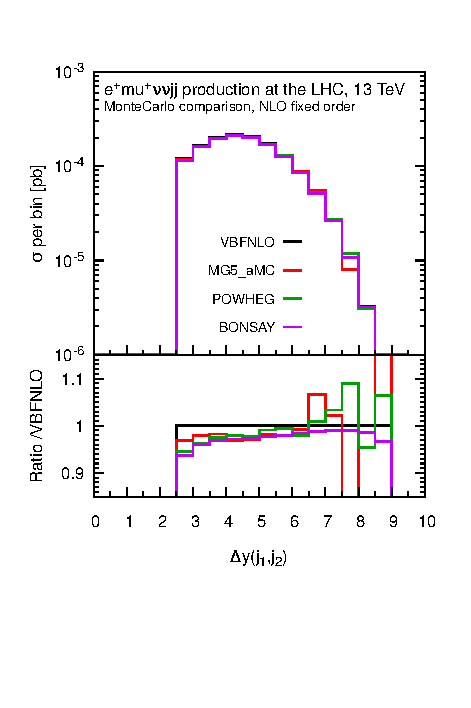
\includegraphics[width=0.4\textwidth,angle=0,clip=true,trim={0.4cm 2cm 0.cm 1.cm}]{figures/NLO/dyj1j2_NLO.pdf}
\caption{\label{fig:distNLO1} Differential distributions in the invariant mass (top) and rapidity difference of the two tagging jets (bottom).
The LHC process considered is ${\rm p}{\rm p}\to\mu^+\nu_\mu{\rm e}^+\nu_{\rm e}{\rm j}{\rm j}$ at NLO accuracy and order $\mathcal{O}(\alpha_{\rm s}\alpha^6)$.
The description of the different programs used can be found in Sec.~\ref{subsec:codedescr}.
The upper plots provides the absolute value for each prediction while the lower plots presents all predictions normalised to {\sc MoCaNLO}+{\sc Recola} which is one of the full predictions.
The predictions are obtained in the fiducial region described in Sec.~\ref{subsec:inputpar}.
\MP{MG statistics should be improved and the baseline changed to Recola.}
}
\end{figure*}

Concerning the transverse momentum (top) and rapidity (bottom) of the hardest jet shown in Fig.~\ref{fig:distNLO2}, the situation is rather different.
While {\sc MadGraph5\_aMC\-@NLO} is very close to the full prediction for low transverse momentum, it is diverging from it at larger transverse momentum.
This is in contrast with {\sc Bonsay} and {\sc Powheg} which approximate the full computation reasonably well over the whole range and in particular in the high transverse-momentum region.
Finally, {\sc VBFNLO} predicts higher rates over the whole range apart from around $200\GeV$ where it is in perfect agreement with the complete calculation.
Concerning the rapidity of the hardest jet, {\sc VBFNLO} is in good agreement with {\sc MoCaNLO}+{\sc Recola} in the rapidity range $|y_{j_1}| < 3$.
For larger rapidity, the other codes constitute a better description of the full process at order $\mathcal{O}(\alpha_{\rm s}\alpha^6)$.

 \begin{figure*}[hbt!]
   \centering
   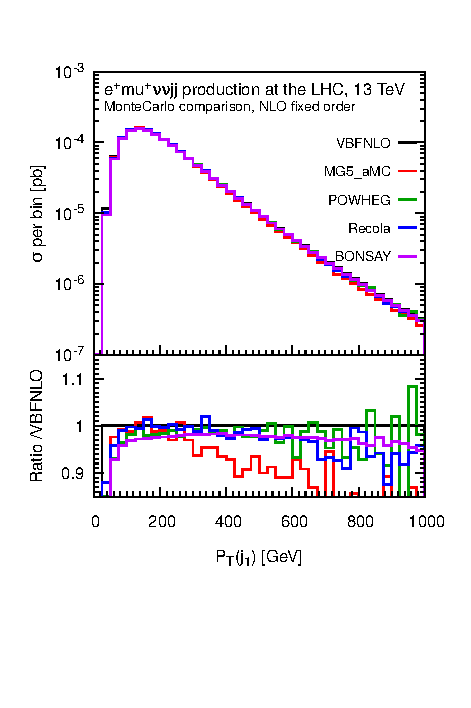
\includegraphics[width=0.4\textwidth,angle=0,clip=true,trim={0.4cm 2cm 0.cm 1.cm}]{figures/NLO/ptj1_NLO.pdf}
   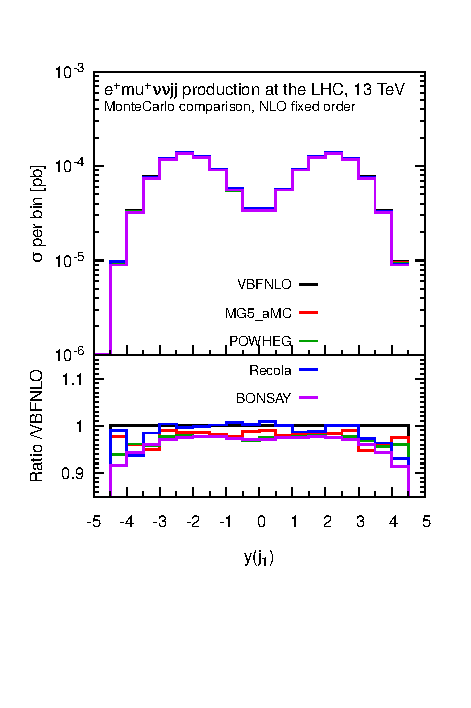
\includegraphics[width=0.4\textwidth,angle=0,clip=true,trim={0.4cm 2cm 0.cm 1.cm}]{figures/NLO/yj1_NLO.pdf}
\caption{\label{fig:distNLO2} Differential distributions in the transverse momentum (top) and rapidity of the hardest jet (bottom).
The LHC process considered is ${\rm p}{\rm p}\to\mu^+\nu_\mu{\rm e}^+\nu_{\rm e}{\rm j}{\rm j}$ at NLO accuracy and order $\mathcal{O}(\alpha_{\rm s}\alpha^6)$.
The description of the different programs used can be found in Sec.~\ref{subsec:codedescr}.
The upper plots provides the absolute value for each prediction while the lower plots presents all predictions normalised to {\sc MoCaNLO}+{\sc Recola} which is one of the full predictions.
The predictions are obtained in the fiducial region described in Sec.~\ref{subsec:inputpar}.
\MP{MG statistics should be improved and the baseline changed to Recola.}
}
\end{figure*}

The last set of differential distributions is the invariant mass of the two charged lepton (top) and the Zeppenfeld variable for the anti-muon (bottom).
Concerning the comparison of the predictions, both distributions display a rather similar behaviour.
Indeed, the hierarchy mentioned previously is here respected and enhanced towards high invariant mass or high Zeppenfeld variable.
{\sc MoCaNLO}+{\sc Recola} and {\sc VBFNLO} are in rather good agreement for both distributions for the kinematic range displayed here.
The other three VBS approximations are close to each other within few per cent.

 \begin{figure*}[hbt!]
   \centering
   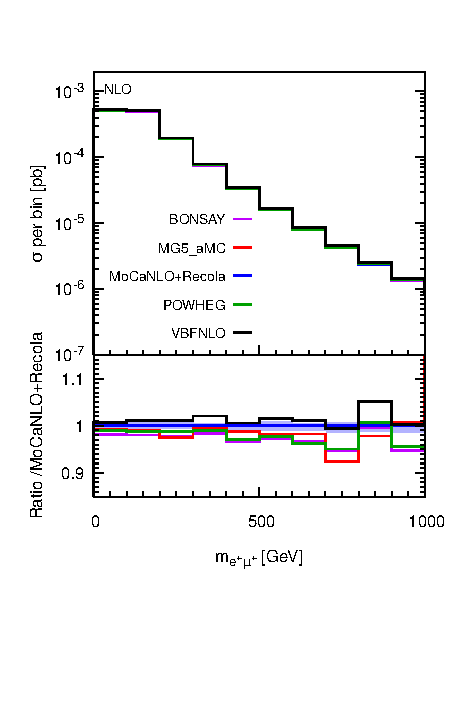
\includegraphics[width=0.4\textwidth,angle=0,clip=true,trim={0.4cm 2cm 0.cm 1.cm}]{figures/NLO/mll_NLO.pdf}
   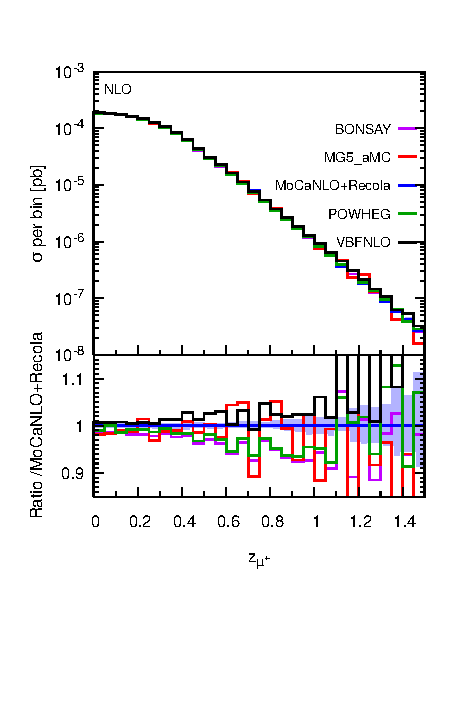
\includegraphics[width=0.4\textwidth,angle=0,clip=true,trim={0.4cm 2cm 0.cm 1.cm}]{figures/NLO/zmu_NLO.pdf}
\caption{\label{fig:distNLO3} Differential distributions in the invariant mass of the two charged leptons (top) and Zeppenfeld variable for the muon (bottom).
The LHC process considered is ${\rm p}{\rm p}\to\mu^+\nu_\mu{\rm e}^+\nu_{\rm e}{\rm j}{\rm j}$ at NLO accuracy and order $\mathcal{O}(\alpha_{\rm s}\alpha^6)$.
The description of the different programs used can be found in Sec.~\ref{subsec:codedescr}.
The upper plots provides the absolute value for each prediction while the lower plots presents all predictions normalised to {\sc MoCaNLO}+{\sc Recola} which is one of the full predictions.
The predictions are obtained in the fiducial region described in Sec.~\ref{subsec:inputpar}.
\MP{MG statistics should be improved and the baseline changed to Recola.}
}
\end{figure*}
